%----------------------------------------------------------------------------------------
%	PACKAGES AND OTHER DOCUMENT CONFIGURATIONS
%----------------------------------------------------------------------------------------

\documentclass[a0,portrait]{a0poster}

\usepackage{multicol} % This is so we can have multiple columns of text side-by-side
\columnsep=100pt % This is the amount of white space between the columns in the poster
\columnseprule=3pt % This is the thickness of the black line between the columns in the poster

\usepackage[svgnames]{xcolor} % Specify colors by their 'svgnames', for a full list of all colors available see here: http://www.latextemplates.com/svgnames-colors

\usepackage{times} % Use the times font
%\usepackage{palatino} % Uncomment to use the Palatino font

\usepackage{graphicx} % Required for including images
\graphicspath{{figures/}} % Location of the graphics files
\usepackage{booktabs} % Top and bottom rules for table
\usepackage[font=small,labelfont=bf]{caption} % Required for specifying captions to tables and figures
\usepackage{amsfonts, amsmath, amsthm, amssymb} % For math fonts, symbols and environments
\usepackage{wrapfig} % Allows wrapping text around tables and figures
\usepackage[all]{xy} %Allows arrow diagrams

\begin{document}

%----------------------------------------------------------------------------------------
%	POSTER HEADER 
%----------------------------------------------------------------------------------------

% The header is divided into two boxes:
% The first is 75% wide and houses the title, subtitle, names, university/organization and contact information
% The second is 25% wide and houses a logo for your university/organization or a photo of you
% The widths of these boxes can be easily edited to accommodate your content as you see fit

\begin{minipage}[b]{0.75\linewidth}
\veryHuge \color{NavyBlue} \textbf{Homestyle From a Distance} \color{Black}\\ % Title
\Huge\textit{Representation and Constituency Emphasis in the European Parliament}\\[2cm] % Subtitle
\huge \textbf{Jeffrey Ziegler}\\[0.5cm] % Author(s)
\huge Washington University in St. Louis\\[0.4cm] % University/organization
\end{minipage}

%----------------------------------------------------------------------------------------

\begin{multicols}{2} % This is how many columns your poster will be broken into, a portrait poster is generally split into 2 columns

%----------------------------------------------------------------------------------------
%	OVERVIEW
%----------------------------------------------------------------------------------------

\color{SaddleBrown} % SaddleBrown color for the introduction

\section*{Overview}

Electoral systems represent a powerful institutional consideration for politicians because they frame the manner in which voters select winning candidates. Electoral characteristics, such as ballot structure, create \textit{personal voting seeking incentives} that ultimately shape the manner in which politicians compete for votes and interact with constituents (Duverger, 1954; Rae, 1967; Taagepera \& Shugart, 1989; Cox, 1997). We hypothesize that ballot structures which reinforce personal interactions between representatives and citizens result in homestyle practices that entice legislators to attend less roll-call votes in the European Parliament (EP). Yet, when Members of the EP (MEPs) attend plenary sessions, they are more likely to engage in personally rewarding behavior such as participating in floor debates.

%----------------------------------------------------------------------------------------
%	OBJECTIVES
%----------------------------------------------------------------------------------------

\color{DarkSlateGray} % DarkSlateGray color for the rest of the content

\section*{Main Objectives}

The primary concern with this section of the project is to determine which MEPs are most likely to participate voluntarily during plenary sessions in an effort to gain visible, personalized attention. To do so, we first determined which activities MEPs could claim personal political recognition for during debates throughout the 7th EP (2009-2014). Such actions include:

\begin{itemize}
\item \textit{Submitting a question for oral response to the Commission}: Highlight an area of concern apart from one's party group.
\item \textit{Invoke the "catch-the-eye" procedure}: Allows MEPs to breakaway from party group talking points and discuss more personal opinions on floor during debate session.
\end{itemize}

In contrast, an example of "party focused" behavior includes:

\begin{itemize}
\item \textit{Relay party message}: MEPs speak in a debate on behalf of their party.
\end{itemize}

%----------------------------------------------------------------------------------------
%	MATERIALS AND METHODS
%----------------------------------------------------------------------------------------

\section*{Materials and Methods}

The content of plenary debates are found within session minutes. To obtain the content of submitted documents and debate speeches, one must first identify when a debate has occurred. Once a debate is catalogued within the minutes, the script identifies if any requests for oral answer are submitted, and if so, the contents and author are pulled. Next, the script establishes whether an MEP invoked the catch-the-eye procedure, and if so, it gathers the content of their speech.

\begin{displaymath}
\xymatrix{\text{Plenary session} \ar[r] & \text{Debate} \ar[dr] \ar[d] \\
& \text{Request for oral answer} \ar[d] & \text{Catch-the-eye} \ar[d] \\
& \text{Content \& Name} & \text{Content \& Name}}
\end{displaymath}

%
\begin{center}\vspace{1cm}
\begin{tabular}{l l l l}
\toprule
\textbf{Date} & \textbf{Catch-the-eye} & \textbf{Debate}\\
\midrule
Thursday, 17 April 2014�&  Spyros Danellis &  4. Shipments of waste ***I (debate) \\
Thursday, 17 April 2014 &   Seán Kelly &  19. Infringements of competition law (debate) \\
Thursday, 17 April 2014 &   Theodor Dumitru Stolojan &  19. Infringements of competition law (debate) \\
Wednesday, 16 April 2014 & NA & 20.�European long-term investment funds(debate) \\
\bottomrule
\end{tabular}
\captionof{table}{\color{Green} Example of csv-output}
\end{center}\vspace{1cm}
%

\subsection*{Example of debate content}

\textit{4. Shipments of waste ***I (debate) CRE Report on the proposal for a regulation of the European Parliament and of the Council amending Regulation (EC) No 1013/2006 on shipment of waste [COM(2013)0516 - C7-0217/2013- 2013/0239(COD)] - Committee on the Environment, Public Health and Food Safety. Rapporteur: Bart Staes (A7-0069/2014)\\
Bart Staes introduced the report.\\
The following spoke: Janez Potočnik (Member of the Commission).}\\
\textbf{The following spoke}: \textit{Karl-Heinz Florenz, on behalf of the PPE Group, Marusya Lyubcheva, on behalf of the S\&D Group, Gerben-Jan Gerbrandy, on behalf of the ALDE Group, Anna Rosbach, on behalf of the ECR Group, Sabine Wils, on behalf of the GUE/NGL Group, Jaroslav Paška, on behalf of the EFD Group, Judith A. Merkies and �?sa Westlund.}\\
\textbf{The following spoke under the 'catch-the-eye' procedure: Spyros Danellis.}\\
\textit{The following spoke: Janez Potočnik and Bart Staes.\\
The debate closed.\\
Vote: minutes of 17.4.2014, item 9.8.\\
Last updated: 3 June 2014Legal notice}

\subsection*{Example of catch-the-eye procedure}

\textit{Andrew Henry William Brons (NI). - Mr President, there is a principle in English civil law called ?to one who is willing, no harm is done?. In other words, you cannot sue if you put yourself in danger of loss or injury. These illegal immigrants were not kidnapped in their own countries by wicked Europeans who then brought them to Europe and incarcerated them for eighteen months or more. They chose to enter an EU country illegally and then avoided being repatriated. Presumably they are free to return to their countries of origin, but refuse to do so.}

%----------------------------------------------------------------------------------------
%	RESULTS 
%----------------------------------------------------------------------------------------

\section*{Results}

The frequential distribution pertaining to the daily prevalence of the catch-the-eye procedure reveals its relatively persistent use. However, though the procedure is invoked regularly, we can see by the second figure that very few MEPs are habitual users of the catch-the-eye procedure and very rarely do so more than 50 times during a five year term.

\begin{center}\vspace{1cm}
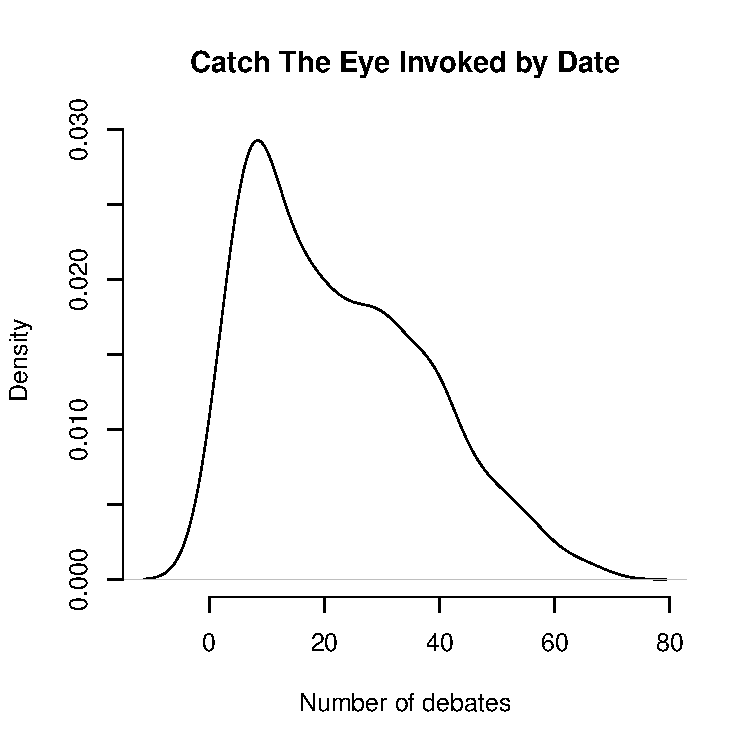
\includegraphics[width=0.8\linewidth]{catchDate.pdf}
\end{center}\vspace{1cm}

\begin{center}\vspace{1cm}
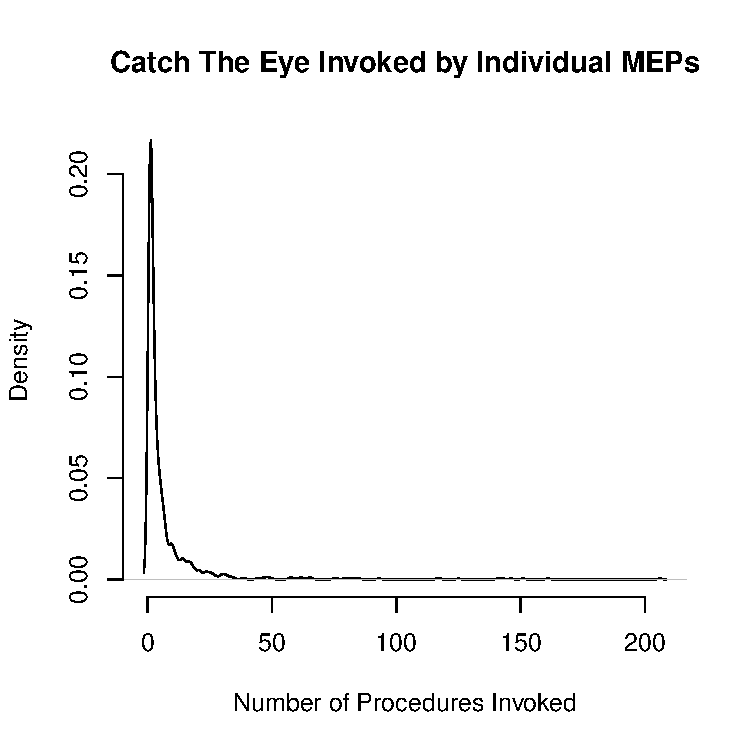
\includegraphics[width=0.8\linewidth]{catchMEP.pdf}
\end{center}\vspace{1cm}

%----------------------------------------------------------------------------------------
%	FORTHCOMING RESEARCH
%----------------------------------------------------------------------------------------

\section*{Forthcoming Research}

Moving forward, we will need to determine:

\begin{itemize}
\item How to approach the issue of text analysis. What elements of debates/speeches are most important to capture whether MEPs make an effort to gain personal "credit" or discuss their constituencies.
\item Are there strategic motivations of using other types of procedures that could result in credit taking (ex. asking a question by \textit{issuing a blue card} to another MEP who has the floor during a plenary speech).
\end{itemize}

%----------------------------------------------------------------------------------------

\end{multicols}
\vspace{2cm}
\begin{center}
\begin{minipage}[b]{0.25\linewidth}

\includegraphics[width=20cm]{washUlogo.jpg}\\
\end{minipage}
\end{center}
\end{document}